\section{Related Work}

\subsection{Navigation Planning Robotics}
Chestnut, 2007, designed the Adaptive Action Model that uses a search algorithm based on its suitability to the current environment. On obstacle-free, flat ground, the planner uses action set directly as the set of actions for node expansion. In the presence of rough terrain or obstacles, the algorithm performs a local search around $x\prime$ to find a new state, $x\prime\prime$, and compute a new action to reach that state, $a\prime$. This approach provides multiple local search mechanisms to drive footstep planning. This is important in the case of an inchworm, especially when we navigate around obstacles. While this approach uses multiple options, it does not guarantee optimality. Optimality is an important consideration in the light of swarm construction as this involves multiple robots. In order to allow each robot to behave efficiently, we need to provide close to optimal paths for navigation \cite{LeggedRobotsNavPlanning}.

\subsection{Swarm Scaffolding MQP}

\begin{figure}[ht]
    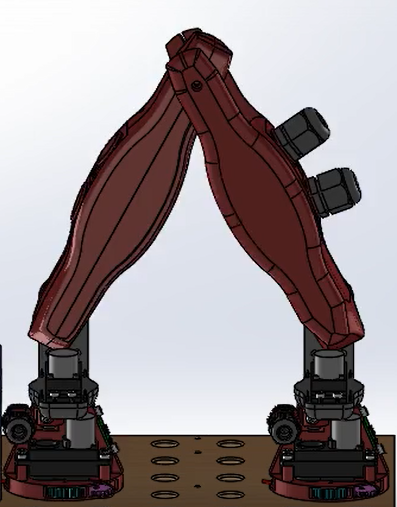
\includegraphics[width=\linewidth]{figures/InchwormPic.PNG}
    \caption{SolidWorks model of the inchworm robot developed by the MQP \cite{PastMQP}}
    \label{fig:Inchworm}
\end{figure} 

The previous iteration of this project (Swarm Scaffolding) developed the inchworm robot design (see \autoref{fig:Inchworm}) and rudimentary motion planning to navigate the workspace area. The robot’s dimensions and gait are based on this design. The team developed a novel Face* algorithm to go from block A to block B within the structure. This is a 3D adaptation of A* and in addition, accounts for reachability of the end effector. The algorithm models each step as two types: (1) a step that results in different orientations between the end effectors; (2) a step that results in the same orientations between the end effectors. The algorithm filters out faces (nodes) based on whether they match the base orientation. Although this algorithm is complete, it does not guarantee optimality\cite{PastMQP}.

\subsection{BILL-E}
BILL-E is a 2019 MIT project that attempts to solve a similar project statement as ours - create a multi-robot construction system. To reach this goal, they use voxels (basic blocks) and inchworm-inspired robots. Their success in efficient building is due to their simple motion-planning algorithm which is based on counting the steps the robot takes around the structure. While this helps the robot know where it is with relation to the structure, it poses a drawback - the robot can not leave the structure and a human must add the next block to the structure. Therefore if the robot is detached from the structure, it will not know where it is or how to continue construction. In our project, we propose that the inchworm will ferry the building material from a quarry to the structure, allowing for a better replica of a construction site layout\cite{BillE}.